% ---------------------------------------------------------------------------
% McpRisk v5 -- policy-grade static severity scoring for MCP servers.
% AAMAS 2027 format (26th ICAAMAS, 3-7 May 2027, JW Marriott Hanoi, Vietnam).
%
% AAMAS uses the ACM `acmart' class in sigconf mode with the IFAAMAS copyright
% block. Section numbering is arabic by default here (1, 1.1, 1.1.1) -- no
% override needed, unlike IEEEtran.
%
% Overleaf: upload this folder, compiler pdfLaTeX, main document main.tex.
% `acmart' and ACM-Reference-Format.bst ship with Overleaf's TeX Live.
%
% SUBMISSION vs CAMERA-READY -----------------------------------------------
% AAMAS main-track review is double-blind. For submission, switch the class
% option line below to the `anonymous' variant and keep \settopmatter{
% printfolios=true} so reviewers get page numbers. Confirm the page limit and
% anonymity policy against the AAMAS 2027 submission instructions when they
% are published (deadline listed as early Oct 2026, TBC).
% ---------------------------------------------------------------------------

% -- SUBMISSION (double-blind, page numbers on):
% \documentclass[sigconf, anonymous, review]{acmart}
% \settopmatter{printacmref=false, printfolios=true}

% -- CAMERA-READY / working draft (current):
\documentclass[sigconf]{acmart}
\settopmatter{printacmref=false}

% AAMAS boilerplate: no ACM reference block, no copyright footnote, no running
% headers. These three lines are prescribed by the IFAAMAS template.
\renewcommand\footnotetextcopyrightpermission[1]{}
\pagestyle{plain}

% NOTE ON \setcopyright: the AAMAS template prescribes \setcopyright{ifaamas},
% but `ifaamas' is NOT a value in the stock acmart.cls -- it only exists in the
% patched acmart.cls that IFAAMAS ships inside the official AAMAS template
% bundle. Compiling against stock acmart with it raises
%   "Package xkeyval Error: value `ifaamas' is not allowed."
% So this draft uses a stock-safe value. When you drop the official AAMAS
% bundle's acmart.cls into this folder, swap the two lines below.
% \setcopyright{ifaamas}
\setcopyright{rightsretained}

\acmConference[AAMAS '27]{Proc.\ of the 26th International Conference on
Autonomous Agents and Multiagent Systems (AAMAS 2027)}{May 3 -- 7,
2027}{Hanoi, Vietnam}
\acmYear{2027}
\copyrightyear{2027}
\acmDOI{}
\acmPrice{}
\acmISBN{}
\acmSubmissionID{}

% --------------------------------------------------------------- packages ---
% acmart already loads amsmath, booktabs, graphicx and xcolor -- loading
% amssymb on top of it clashes with \Bbbk from the Libertine math setup.
\usepackage{balance}
\usepackage{enumitem}   % optional args on enumerate (contributions list)

% ---------------------------------------------------------------- shortcuts ---
\newcommand{\eg}{e.g.,\ }
\newcommand{\ie}{i.e.,\ }
% \newcommand{\framework}{\textsc{McpRisk}}

% Placeholder marker for sections not yet written. Delete the macro once the
% skeleton is filled in; it renders visibly so nothing ships by accident.
\newcommand{\stub}[1]{\textit{\textcolor{gray}{[To be written: #1]}}}


% \newcommand{\frameworkname}{\textsc{CARMA\xspace}}
\newcommand{\frameworkname}{\textsc{CARMA}}

\begin{document}

% ------------------------------------------------------------------- title ---
\title{Risk-Aware MCP: Risk Assessment for Model Context Protocol Invocations}

\author{Tomer Ovadya}
\affiliation{%
  \institution{Ben-Gurion University of the Negev}
  \department{Software and Information Systems Engineering}
  \city{Beer-Sheva}
  \country{Israel}}
\email{ovadyat@post.bgu.ac.il}

\author{Asaf Shabtai}
\affiliation{%
  \institution{Ben-Gurion University of the Negev}
  \department{Software and Information Systems Engineering}
  \city{Beer-Sheva}
  \country{Israel}}
\email{shabtaia@bgu.ac.il}

\renewcommand{\shortauthors}{Ovadya and Shabtai}

% ---------------------------------------------------------------- abstract ---
\begin{abstract}
% \stub{abstract --- write last, once the evaluation section is fixed.}

Model Context Protocol (MCP) servers expose tools that allow AI agents to interact directly with organizational assets and services. Even legitimate tool invocations can have substantially different consequences depending on the affected asset, the operation performed, and the scope of its effect.

% For example, the same file operation may target a temporary artifact or a critical organizational asset.

Such risk does not require malicious intent: misuse may result from overly broad delegation, incorrect tool or parameter selection. This motivates assessing the risk of a concrete MCP invocation before it is executed.

We present a two-stage framework for MCP risk assessment. At design time, a \textit{Static Scanner} constructs a tool--asset risk surface by combining tool impact, organizational asset sensitivity, and blast radius. At runtime, a \textit{Dynamic Scanner} adapts this baseline using invocation-specific arguments, execution context, and previously observed behavior. We evaluate the framework across 16 deployments derived from nine real MCP tool catalogs, covering 262 tools, 221 assets, and 3,615 candidate tool--asset pairs, together with 3,000 live invocations across GitHub, Slack, and Calendar deployments.


\end{abstract}

% ------------------------------------------------------------ CCS + keywords ---
\begin{CCSXML}
<ccs2012>
   <concept>
       <concept_id>10002978.10003006.10003013</concept_id>
       <concept_desc>Security and privacy~Distributed systems security</concept_desc>
       <concept_significance>500</concept_significance>
       </concept>
   <concept>
       <concept_id>10002978.10002991.10002995</concept_id>
       <concept_desc>Security and privacy~Access control</concept_desc>
       <concept_significance>300</concept_significance>
       </concept>
   <concept>
       <concept_id>10010147.10010178.10010179</concept_id>
       <concept_desc>Computing methodologies~Intelligent agents</concept_desc>
       <concept_significance>300</concept_significance>
       </concept>
 </ccs2012>
\end{CCSXML}

\ccsdesc[500]{Security and privacy~Distributed systems security}
\ccsdesc[300]{Security and privacy~Access control}
\ccsdesc[300]{Computing methodologies~Intelligent agents}

\keywords{Model Context Protocol; AI agents; risk scoring; security
categorization; data classification policy; LLM security; access control}

\maketitle

% ---------------------------------------------------------------------------
% Section 1 -- Introduction (short paper: FLAT, no subsections)
%
% Structure follows the "technical-challenge version 2" template from the
% research-paper-writing skill: our insight has historical roots in a
% traditional line (risk-adaptive access control, 2007-2011), so that line is
% used as conceptual backing before showing why modern MCP defenses still fail.
%
% Paragraph roles:
%   P1 opening    -- agentic applications and MCP
%   P2 direction  -- server as protected asset; misuse through legitimate access
%   P3 challenge  -- RBAC/ABAC answer "may it?", not "how dangerous is it?"
%   P4 challenge  -- risk-based access control already solves this shape, but
%                    not for agents; current MCP defenses remain binary
%   P5 insight    -- what the risk must be computed from (static, dynamic, history)
%   P6 method     -- our methodology
%   P7 evidence   -- implementation, evaluation, three contributions
%
% Budget: ~850 words. Citations: 24 of the 37 in refs.bib.
%
% EXPECTED: \ref to sec:framework / sec:eval typesets as "??" until those
% sections exist. Not a build error.
% ------------------------------------------------------------------------
\section{Introduction}
\label{sec:intro}

AI agents no longer only generate text; they act. They read data, modify files,
update databases, and call external services for their users. The Model Context
Protocol (MCP)~\cite{anthropic2024mcp} standardizes this exchange: a server
publishes tools, and a connected agent discovers and invokes them over
JSON-RPC~\cite{mcp2026spec}. The public server ecosystem is growing quickly~\cite{hou2026mcp}, and audits of deployed servers find recurring weaknesses~\cite{hasan2025firstglance}. An agent's decision
now lands directly on the systems and assets behind those tools. These tools let agent decisions directly affect organizational assets. MCP
standardizes how tools are discovered and invoked, but it does not assess the
risk of a specific call. Its annotations describe the tool rather than the
asset it affects, so a destructive tool receives the same label whether it
targets a temporary file or a production database.

Most MCP and agent security research studies how malicious servers or tools can
harm the agents that use
them~\cite{invariant2025toolpoisoning,shi2025toolhijacker}. Other work audits
MCP server implementations and exposed capabilities for software weaknesses or
excessive privilege~\cite{kumar2026mcpinsos,huang2026auditing}. For example, at runtime,
MTGuard inspects invocation parameters and observed execution to detect policy
violations~\cite{he2026mtguard}. These approaches identify vulnerabilities,
excessive permissions, or unsafe behavior. They do not estimate the consequence
of an authorized invocation from the sensitivity and scope of the asset it
affects. Our work provides this estimate.


We study \emph{misuse}: a legitimate capability used beyond what the task requires~\cite{anderson1980threat}. It needs no malicious agent and no malicious server. It can start with an operator who states a task loosely, delegates too broadly, or grants excess permission~ \cite{owasp2025llm06} . Studies of MCP
applications and servers report broad system access and over-privileged
tools~\cite{li2025privilege,huang2026auditing}. Misuse can also result from
model behavior: an agent may select an available but inappropriate
tool~\cite{yin2025reasoningtrap}, or recognize a risk in general but fail to
account for it during execution~\cite{tang2025riskknowledge}. We do not ask why the agent made the call. We assess what the call can do.
Reading a build log and reading stored credentials may use the same tool, but
the risks are different. We therefore analyze the full invocation: the tool,
the asset it affects, the arguments, the execution context, and the agent's
recent actions.



Access control decides whether a request is allowed. Role and attribute-based
models~\cite{sandhu1996rbac,hu2014abac} evaluate permissions under a policy,
but they do not normally assign a risk level to an allowed request. This gap
also appears in agent frameworks: exposing a tool does not ensure that each call
is authorized using its actual argument values~\cite{mellafe2026capability}.
Authentication identifies the caller, and authorization defines what the caller
may do. Neither measures the possible consequence of a specific authorized
call.


Adding risk to an access-control decision is not new. Early work quantified risk
during authorization~\cite{cheng2007fuzzymls}, and later work incorporated
risk-adaptive access control into an attribute-based
framework~\cite{kandala2011radac}. The area has since been widely
studied~\cite{atlam2020riskbased}. Recent work extends this idea to agents,
using an LLM judge to consider task risk, asset risk, and model
uncertainty~\cite{fleming2025tbac}. However, these models do not define an
MCP-specific consequence score for a concrete invocation based on the tool, the
sensitivity of the affected asset, and the scope of the call.


To our knowledge, no existing method estimates the consequence of a concrete
MCP invocation from the sensitivity and scope of the asset it affects. Many
defenses operate at the agent, client, or middleware layer, where they restrict
available tools or authorize calls before
execution~\cite{shi2025progent,zhu2025miniscope,betser2026agentrim,
li2026conleash,abaev2026agentguardian}. Server-side authorization has also begun
to appear: IGAC checks a proposed call and its payload against the user's
declared intent~\cite{zhu2026igac}. Other runtime systems return safety scores
or decisions such as allow, review, or
block~\cite{yang2026agenttrust,zhang2026stars,hossain2026nexus}. These outputs
indicate whether a call is permitted, suspicious, or requires intervention, but
they do not estimate the severity of an authorized call for the specific
organizational asset it affects.

Consequently, existing vulnerability-scoring frameworks do not address this problem either. CVSS estimates the severity of vulnerabilities in software, hardware, and firmware~\cite{first2023cvss}, while AIVSS extends vulnerability scoring with factors tailored to agentic AI systems~\cite{huang2026aivss}. However, both assess vulnerabilities rather than the potential consequence of a concrete MCP operation on an organizational asset. Our approach instead computes this operation-level consequence and uses it as the basis for subsequent risk-aware decisions.


Risk belongs to a tool--asset pair, not to the tool alone. For example,: \texttt{read\_file} poses little risk when applied to a public document but
substantial risk when applied to regulated data. We therefore compute a
baseline from three factors: tool impact, asset sensitivity, and
\emph{blast radius}, meaning the portion of the asset affected by one call.
The call's arguments may change this baseline, while its context and the
agent's recent activity may indicate whether the call is unusual.

To address this problem, we introduce \textbf{\frameworkname\ } (\textit{Continuous Adaptive Risk Model for MCP Actions}), a framework for assessing the risk of MCP operations on organizational assets.

\frameworkname\ computes risk in two complementary stages. At design time, its \textit{Static Scanner} establishes a baseline risk for each reachable tool--asset pair by combining tool impact, asset sensitivity, and blast radius. Asset sensitivity is derived from the organization's information-classification policy, following established guidance for mapping information types to impact categories~\cite{nist2004fips199,nist2008sp80060}. At request time, the \textit{Dynamic Scanner} adapts this baseline using operation-specific arguments, execution context, and the agent's recent activity. The resulting score can then be compared with organizational policies to support or decline MCP-related actions. In this sense, the score also provides a measurable basis for adjustable autonomy, where control may shift between the agent and a human according to the risk of the current operation~\cite{pynadath2002adjustable}.

We evaluate \frameworkname\ using tool catalogs from real vendor MCP servers together with organizational policies, asset inventories, and concrete invocation scenarios. The evaluation examines both the design-time risk surface produced across tool--asset combinations and the runtime adaptation of these scores as MCP operations are observed.

This paper makes three contributions:
\begin{itemize}
    \item \textbf{Risk-analysis methodology.}
    We introduce a methodology for assessing the misuse risk of MCP operations by combining tool impact, asset sensitivity, blast radius, runtime arguments, execution context, and the agent's recent activity. Asset sensitivity is derived from organizational policy rather than requiring a fully labeled asset inventory.

    \item \textbf{Risk-assessment framework.}
    We develop a framework that implements the proposed methodology through complementary Static and Dynamic Scanners and produces interpretable risk scores.

\item \textbf{MCP-specific evaluation methodology.}
    We introduce an evaluation methodology for MCP risk assessment that systematically constructs organizational environments around real MCP tool catalogs. For each evaluated MCP, we synthesize representative organizational assets and their sensitivity profiles, derive tool--asset combinations according to the exposed tool capabilities, and craft MCP-specific operation scenarios. We further construct time-ordered dynamic scenarios in which usage patterns, scope, frequency, and behavioral history evolve over time, enabling controlled evaluation of both the static risk factors and the dynamic adaptation of the computed risk.
\end{itemize}






% We compute risk at two stages. At design time, we assign a baseline score to
% each tool--asset pair exposed by the server. The score combines tool impact,
% asset sensitivity, and blast radius. Asset sensitivity is derived from
% the organization's information-classification policy, following established
% guidance for mapping information types to impact
% categories~\cite{nist2004fips199,nist2008sp80060}. At request time, we update
% the baseline using the call's arguments, execution context, and the agent's
% recent activity. We compare the resulting score with organizational thresholds
% to approve the call, require human review, or refuse it
% (\S\ref{sec}).

% Adjustable autonomy studies when an agent should act independently and when
% control should pass to a person~\cite{pynadath2002adjustable}. Our score
% provides a measurable basis for this decision. We implement the method as an
% enforcement framework and evaluate it using tool catalogs from real vendor MCP
% servers, together with organizational policies, asset inventories, and
% invocation scenarios (\S\ref{sec}).

% This paper makes three contributions. First, a \textbf{risk-analysis methodology}
% for assessing the misuse risk of an MCP invocation from tool impact, asset
% sensitivity, blast radius, runtime arguments, execution context, and the agent's
% recent activity, deriving asset sensitivity from organizational policy rather
% than from a fully labeled asset inventory. Second, an \textbf{enforcement
% framework} that combines the design-time and request-time assessments and uses
% them to make risk-based access-control decisions for MCP servers. Third, an
% \textbf{evaluation setting} that pairs tool catalogs from real vendor MCP servers
% with synthesized organizational policies, asset inventories, and invocation
% scenarios, used to measure whether the calculated risk levels match
% organizational judgment and whether runtime arguments and behavioral history
% affect the score as intended.
% ---------------------------------------------------------------------------
% Section 2 -- Related Work (short paper: FLAT, four thematic strands)
%
% Not a paper list. Four strands, each one paragraph, each closing on the
% sentence that says why that strand does not answer our question. Bold run-in
% headings instead of \subsection -- subsections cost vertical space and invite
% padding (WRITING-GUIDE.md sec. 7).
%
% Paragraph roles:
%   P1 (a) MCP security        -- the field protects the agent from the server
%   P2 (b) agent/MCP defenses  -- they end at an enforcement verdict
%   P3 (c) access control      -- KEY STRAND: RBAC/ABAC permit; risk-adaptive
%                                 access control conditions on a computed risk
%                                 value. fleming2025tbac is the NEAREST work and
%                                 is named as such -- the gap is the *input*
%                                 (a decomposed per-invocation estimate), not
%                                 the absence of any risk value for agents.
%   P4 (d) risk scoring        -- scores the server, the tool, or the log
%
% Deliberately NOT repeated here (sec. 1 and sec. 3 already carry it, with the
% same keys): the four-route misuse taxonomy -- yin2025reasoningtrap,
% tang2025riskknowledge, zhan2024injecagent, lynch2025misalignment. P2's job is
% what the defenses *produce*, not why they are needed.
%
% Budget: 600-700 words, ~31 citation keys, all from refs.bib.
% ---------------------------------------------------------------------------
\section{Related Work}
\label{sec:related}

\textbf{MCP Server Security and Risk Assessment.}
Prior work surveys security risks across the MCP
ecosystem~\cite{hou2026mcp} and audits open-source MCP servers for
software weaknesses, MCP-specific vulnerabilities, and maintainability
problems~\cite{hasan2025firstglance}. Several studies examine attacks in which
a malicious server, tool description, or external input influences the
agent~\cite{invariant2025toolpoisoning,shi2025toolhijacker,
zhao2025parasites}. We study the opposite direction: an agent sends a call that
may harm the MCP server or an organizational asset reached through it.
Server-to-agent attacks are outside our scope. We assume only that each tool
performs the operation represented by its declared interface and asset
mapping.

Other work examines the capabilities and weaknesses of MCP servers. Li et al.
analyze 2,562 MCP applications and measure their use of file, network, system,
and memory APIs~\cite{li2025privilege}. Huang et al. combine static pattern
matching with sandboxed execution to detect capabilities such as file access,
network requests, and command execution~\cite{huang2026auditing}. MCP-in-SoS
scans 222 server repositories for code weaknesses, maps them to CWE and CAPEC
entries, and derives repository-level risk from the likelihood and severity
those catalogs assign~\cite{kumar2026mcpinsos}. All three assess the server as
an artifact, independently of the assets a given installation holds, so the
same server receives the same assessment wherever it is deployed.

ConLeash checks whether an MCP call stays within an approved consent boundary~\cite{li2026conleash}. However, it does not estimate the risk or possible impact of a call that is already allowed. Our work addresses this gap by assessing the risk of each invocation from the server side.




\textbf{Defenses for MCP and tool-using agents.}
IGAC checks whether an MCP invocation and its arguments remain within the user's stated intent, while MTGuard compares invocation parameters, runtime behavior, and results against safety policies~\cite{zhu2026igac,he2026mtguard}. Progent and MiniScope enforce least-privilege authorization, whereas AgentGuardian learns admissible tool inputs and invocation sequences from normal executions~\cite{shi2025progent,zhu2025miniscope,abaev2026agentguardian}. These systems check whether a tool call follows the user's request, the security policy, or the agent's normal behavior. However, a call can pass all these checks and still cause serious damage. For example, an agent may be allowed to delete files, but deleting a temporary file and deleting a critical production file do not have the same risk; our work measures this difference at the MCP server.

\textbf{Access control.}
RBAC assigns permissions through roles, while ABAC evaluates attributes of the
caller, asset, requested action, and environment
conditions~\cite{sandhu1996rbac,hu2014abac}. These models can express
fine-grained policies, but they do not directly estimate the possible
consequence of a permitted request.

Risk-adaptive access control adds a calculated risk value to the authorization
decision~\cite{cheng2007fuzzymls}. Kandala et al. place risk within an
attribute-based framework, but leave the concrete risk-calculation method
outside their scope~\cite{kandala2011radac}. Ni et al. use fuzzy rules over
subject and object security information to estimate the risk of an access
operation~\cite{ni2010fuzzy}. Shaikh et al. dynamically calculate trust and
risk for each subject--object pair from the user's past
behavior~\cite{shaikh2012dynamic}. Atlam et al. survey the wider family of
risk-based access-control models~\cite{atlam2020riskbased}.

For agentic systems, Fleming et al. use an LLM judge to create a task policy,
combine static risk values for its tools and assets, and estimate
uncertainty~\cite{fleming2025tbac}. A limitation is that risk is computed for
the whole task and is not updated for each call. For example, reading one
database record and exporting a full table may use the same tool risk value.
Our work instead scores each MCP invocation using its runtime details.

\textbf{Risk scoring for MCP and agents.}
CVSS scores the severity of software vulnerabilities. A study of 196 evaluators
applying CVSS v3.1 found differences between evaluators, and a follow-up found
that 68\% assigned a different severity level to vulnerabilities they had
scored before~\cite{first2023cvss,wunder2024cvss}. AIVSS extends vulnerability
scoring to agentic AI systems~\cite{huang2026aivss}. These frameworks score
vulnerabilities rather than concrete tool calls.

FIPS 199 and NIST SP 800-60 classify information types and systems by the
potential impact of losing confidentiality, integrity, or
availability~\cite{nist2004fips199,nist2008sp80060}. These classifications
provide an organizational view of consequence that our method uses when
assessing the asset affected by a call.

Work closer to our setting studies risk at different stages. MCP-in-SoS scores
weaknesses in an MCP server repository~\cite{kumar2026mcpinsos}, while
AgenTRIM assigns risk levels to tools and applies stronger checks to riskier
ones~\cite{betser2026agentrim}. STARS scores proposed skill invocations using
the request, capability, and runtime context before
execution~\cite{zhang2026stars}. Owiredu-Ashley instead grades the harm of
actions recorded after execution~\cite{owireduashley2026severity}. Together,
These methods answer different risk questions: they assess server weaknesses,
tool capabilities, invocation safety, or harm after execution. They do not
provide a common measure of the consequence to the organization affected by
the call. For example, deleting a temporary cache and deleting payroll records
may use the same tool and both be irreversible, but their organizational impact
is very different. Our work connects each MCP call to the organization's
asset policy and estimates its risk before execution.
% ===========================================================================
% 3. Problem Setting and Threat Model
% ===========================================================================
\section{Threat Model}
\label{threatmodel}

We consider an organizational MCP deployment in which an MCP server exposes tools that allow AI agents to interact with organizational assets and external services. An agent selects a tool and provides concrete arguments, and the MCP server performs the corresponding operation on the reachable asset. We assume that the MCP server and its advertised tools are benign and operate according to their declared functionality. Our protected environment consists of the organizational assets and services reachable through these tools.

Our threat model focuses on \emph{misuse of legitimate MCP capabilities}. Misuse occurs when an MCP operation creates potentially harmful consequences for organizational assets or services, regardless of whether the operation originates from benign error, excessive delegation, compromised behavior, or malicious intent. The operation may still be syntactically valid and supported by the exposed tool. The risk depends on what operation is performed, which asset it affects, how broadly it can affect that asset, and how the capability is exercised at runtime. In contrast to attacks that compromise the MCP server or introduce malicious tools, misuse can arise when a valid MCP operation produces consequences that are inappropriate for the current organizational context.

% We consider several complementary misuse vectors. First, \emph{operation misuse} occurs when an agent selects a capability whose effect is unnecessarily consequential for the task, such as modifying or deleting state when a read operation would suffice. Second, \emph{asset misuse} occurs when an otherwise legitimate capability is applied to an asset with substantially greater organizational sensitivity than expected. The same tool can therefore have very different consequences depending on whether it operates on a temporary artifact or a critical organizational asset. Third, \emph{scope misuse} occurs when an operation affects a broader portion of an asset than necessary, including collections, repositories, user groups, or multiple dependent assets. Fourth, \emph{parameter misuse} arises when concrete argument values expand the impact of an otherwise expected operation. Finally, \emph{behavioral misuse} captures changes in how a capability is exercised over time, such as unusual frequency, previously unseen tool--asset combinations, abrupt changes in targets or scope, or deviations from established operation sequences.

% These misuse vectors are not mutually exclusive. A single operation may, for example, invoke a state-changing tool on a highly sensitive asset, use arguments that broaden its scope, and occur in a pattern not previously observed. Our objective is therefore not to classify the agent as benign or malicious, nor to infer the human user's underlying intent. Instead, we assess the risk associated with carrying out the requested MCP operation from evidence observable or resolvable at the server side.

At design time, this evidence includes the semantics of the exposed tools, the organizational assets they can reach, the sensitivity of those assets, and the scope that an operation can affect. At runtime, additional evidence becomes available from the concrete arguments and execution context.

Common security threats, including malicious MCP servers, tool poisoning, authentication bypass, implementation vulnerabilities, manipulation of organizational policies, and server-to-agent attacks, are outside the scope of this work.


% We assume that the organizational asset information and classification policies used by the framework are trusted and sufficiently accurate for risk assessment, and that the MCP deployment can determine or approximate the asset or asset scope reachable by an operation. We further assume that invocation metadata required by the runtime assessment can be observed and that relevant history can be maintained.


% The following threats are outside our scope: malicious or compromised MCP servers, tool-description poisoning, authentication bypass, exploitation of software vulnerabilities in the MCP implementation, manipulation of the organizational classification policy itself, and attacks originating from a malicious MCP server toward the agent. Our framework also does not attempt to determine whether an operation satisfies the user's semantic intent; rather, it estimates the potential organizational risk of executing the operation given the affected capability, asset, scope, and runtime context.



% \section{Problem Setting and Threat Model}
% \label{sec:threat}

% \subsection{Problem Setting}

% We consider an MCP server operating under normal conditions and exposing a set of tools to agentic applications. An MCP client discovers the tools exposed by the server, including their descriptions and input schemas. When an application selects a tool for execution, the client sends a tools/call request containing the tool name and concrete arguments to the server~\cite{mcp2026spec}. The server processes the request and performs the corresponding operation on the external system or organizational asset accessible through that tool.

% We treat the benign MCP server as the protected party. Our concern is not
% whether an agent is authorized to invoke a tool, but the consequence of an
% operation that has already been permitted.


% At the protocol boundary, the server directly observes the requested tool and
% its arguments. Depending on the deployment, it may also associate the request
% with an authenticated caller or application and resolve the organizational
% asset targeted by the operation.


% \subsection{Threat Model}

% Protocol-valid invocations that have already passed the server's existing
% access-control checks. Malicious MCP servers, tool poisoning, authentication
% bypass, implementation vulnerabilities, and attacks originating from the
% server toward the agent are outside our scope.

% Our concern is that an authorized operation can nevertheless carry substantial
% risk. A permitted call may expose sensitive information, modify important
% state, affect a large organizational scope, or perform an irreversible action.
% Agents may also issue risky calls because of task misunderstanding, incorrect
% tool or parameter selection, or failures to act on available risk information
% ~\cite{yin2025reasoningtrap,tang2025riskknowledge}. Such calls may remain
% authenticated, schema-conforming, and authorized at the MCP boundary.

% We therefore do not attempt to determine whether a call is malicious,
% mistaken, or consistent with the user's intent. Instead, we assess the risk of
% the operation that the MCP server is being asked to perform. The calling agent
% is thus treated as a source of potentially risky requests rather than as an
% assumed adversary.


% \subsection{Assessment Problem}

% We represent the information available for assessing an invocation as

% \begin{equation}
% c=\langle i,t,a,x,h\rangle,
% \label{eq:invocation}
% \end{equation}

% where $i$ identifies the calling agent, application, or credential; $t$ is the
% requested tool; $a$ is the organizational asset targeted by the operation;
% $x$ contains invocation-specific information, including the concrete
% arguments and request-time context; and $h$ denotes relevant previously
% observed invocation history. The target $a$ need not be supplied explicitly by
% the client and may instead be resolved from the tool, its arguments, and the
% server configuration.

% Existing access control first determines whether the invocation is permitted.
% We consider only calls for which

% \begin{equation}
% \mathrm{perm}(c)=1.
% \end{equation}

% For such calls, our objective is to compute, before execution, a graded risk
% assessment

% \begin{equation}
% \rho(c),
% \end{equation}

% representing the risk associated with carrying out the requested operation.

% The assessment combines two complementary sources of evidence. The first
% captures the potential consequence of applying tool $t$ to asset $a$. The
% second captures invocation-specific evidence from $x$ and $h$ that may make
% the current use more or less concerning. Section~\ref{sec:framework} realizes
% these components through the Static and Dynamic Scanners, respectively. The
% framework reports risk; subsequent enforcement decisions remain
% organization-specific and outside the scope of this work.



% ===========================================================================
% 4. Methodology
% ===========================================================================

\section{Methodology}
\label{sec:framework}

\subsection{Overview}

The \frameworkname\ framework separates MCP risk assessment into two layers:
\emph{static risk assessment} and \emph{dynamic risk adaptation}. The Static
Scanner estimates the potential consequence of capabilities exposed by an MCP
server before observing their actual use. The Dynamic Scanner subsequently
adapts this baseline using evidence available for a concrete invocation.

This separation reflects the information available at the two stages. Static
properties such as operation semantics, organizational sensitivity, and
reachable scope can be analyzed when the server and organizational policy are
configured. Runtime evidence, such as concrete arguments and previously
observed behavior, becomes available only when an invocation occurs. The
separation also allows relatively expensive semantic analysis to be performed
outside the invocation path while keeping runtime assessment lightweight.

Figure~\ref{fig:risk-architecture} illustrates the overall methodology.

\begin{figure*}[t]
    \centering
    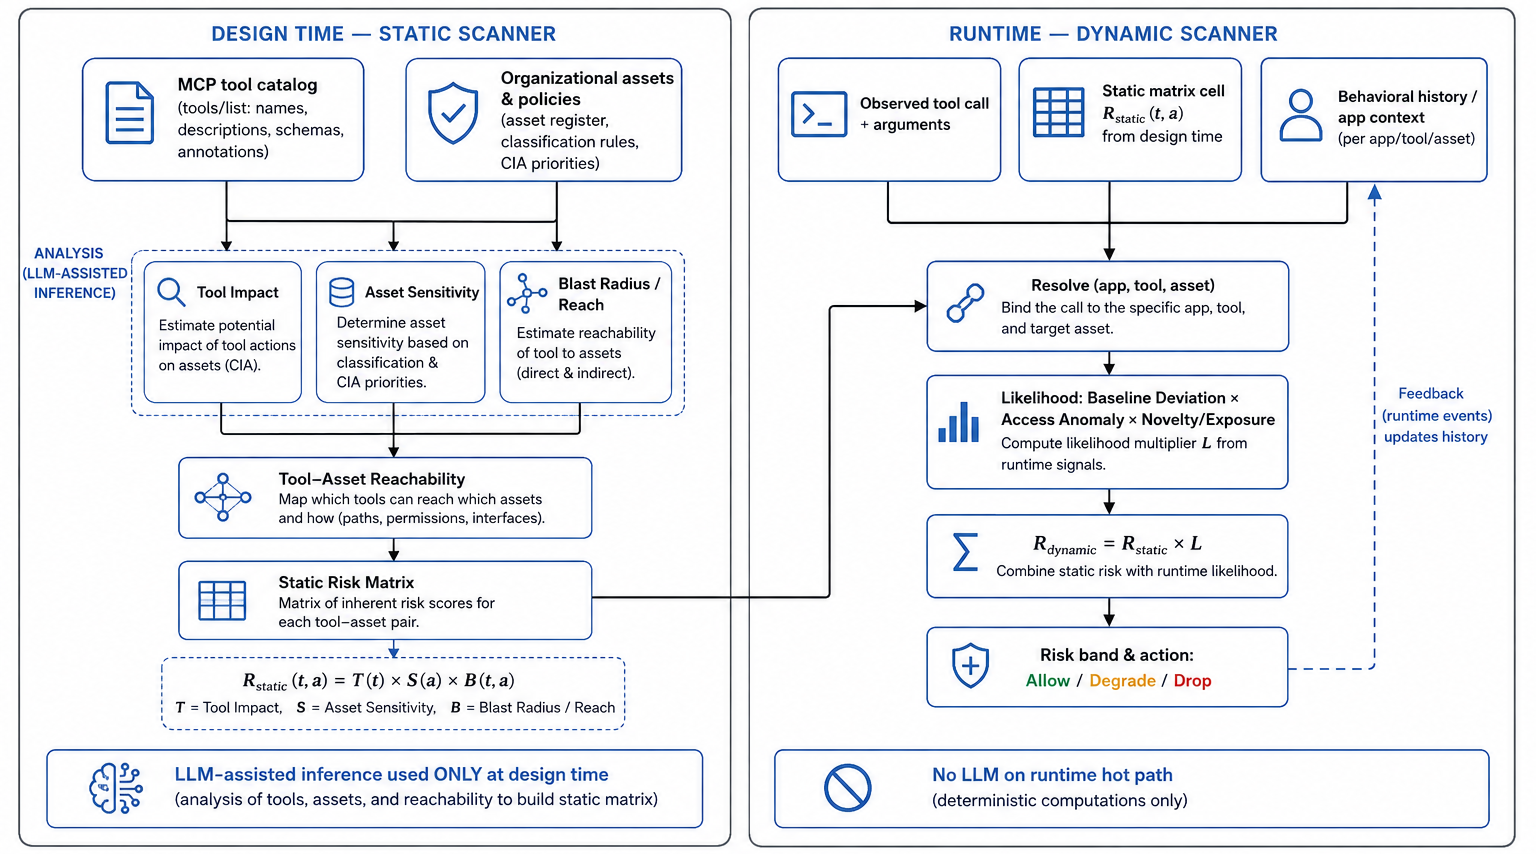
\includegraphics[width=0.95\textwidth]
    {figures/mcp_risk_overall_architecture_updated.png}
    \caption{Overview of the proposed MCP risk-assessment methodology.
    The Static Scanner analyzes MCP tool information and organizational
    assets to construct a tool--asset risk matrix. At runtime, the
    Dynamic Scanner adapts the corresponding baseline using
    invocation-specific and historical evidence.}
    \label{fig:risk-architecture}
\end{figure*}

\frameworkname\ is implemented in Python. Every stage that requires semantic
judgment runs at design time against a locally hosted instruction model
(Qwen2.5-32B served through Ollama) with greedy decoding and a fixed seed, so a
given tool catalog yields a byte-identical risk matrix on re-scan. The runtime
path contains no model call at all.


% ---------------------------------------------------------------------------
\subsection{Invocation Logging}
\label{sec:impl-logging}

Both layers are downstream of one capture mechanism. The Static Scanner
consumes the tool catalog a server advertises; the Dynamic Scanner consumes the
ordered history of invocations against it. We obtain both from the MCP message
stream itself rather than from any server-specific API, SDK hook, or agent
instrumentation.

The design point is that MCP fixes the \emph{message layer} --- every
interaction is a JSON-RPC~2.0 request or response --- while leaving the
\emph{transport} open: a locally spawned server communicates over stdio, and a
hosted or vendor-operated server is reached over HTTP, either as HTTP with
server-sent events or as streamable HTTP~\cite{mcp2026spec}. Capturing at the
JSON-RPC layer rather than at a transport therefore yields one implementation
that covers both local and web-hosted deployments, and requires no cooperation
from the server and no modification to the agent.

We use two collection paths that converge on the same records:

\textbf{Local (stdio).} The server is launched as a subprocess. Requests are
written as line-delimited JSON to its standard input, responses are read from
its standard output, and its standard error is drained on a separate thread so
a chatty server cannot deadlock the pipe. Each request carries a monotonically
increasing identifier and responses are matched back to it by that identifier.

\textbf{Remote (HTTP).} The server is fronted by a recording reverse proxy.
Every HTTP flow is written as one JSON record carrying request and response
bodies, headers, status, and start and end timestamps. Event-stream framing is
unwrapped, so the recovered payload is the same JSON-RPC object that the stdio
path observes directly.

A parser then reconstructs the interaction from the raw stream alone, pairing
requests with responses per session and emitting three tables. The
\emph{catalog} table holds one row per tool advertised in a \texttt{tools/list}
result --- name, description, argument and result schemas, and the
read-only, destructive, and idempotent annotation hints --- and is the input to
the static layer. The \emph{calls} table holds one row per invocation ---
timestamps, elapsed time, tool, argument names, argument values, status or
error, and response --- and is the input to the dynamic layer. The
\emph{sessions} table holds one row per client session, including the
negotiated protocol version and the client and server identities exchanged
during the handshake.

Two details of the reconstruction matter for risk assessment. First, MCP
servers signal failure in two different shapes: a top-level JSON-RPC error
object, and a successful response whose result is flagged as an error with the
message carried in its content. The parser normalizes both, because a rejected
invocation is still evidence about the caller and must not be dropped from the
behavioral history. Second, the parser flags structural anomalies that no
individual call reveals --- sessions that connect but never complete the
handshake, repeated identical invocations within a short window, and calls
whose latency is far above the observed norm.

The tool catalog is recorded exactly as the server advertises it. Even under
the benign-server assumption of Section~\ref{threatmodel}, a tool's declared
annotations and prose remain self-reported and imprecise: the protocol defines
them as hints, and a catalog written for human readers routinely understates
what a tool can reach. The static layer therefore treats the declaration as
evidence to be bounded rather than as ground truth, as described next.


% ---------------------------------------------------------------------------
\subsection{Static Risk Assessment}
\label{sec:static}

The Static Scanner operates over two principal information sources: the MCP
tool catalog and organizational asset information. From the MCP server, it
collects the exposed tool definitions, including names, descriptions, argument
schemas, and available annotations, e.g., through
\texttt{tools/list}~\cite{mcp2026spec}. From the organization, it obtains the
asset register and available classification policy or metadata.

Before assigning a score, the scanner determines whether tool $t$ can operate
on asset $a$. Reachability may follow from tool parameters, configured
roots, repositories, database scopes, API mappings, or organizational
metadata. Pairs that cannot interact are represented as \emph{N/A}, rather
than assigned a low risk score.

For every reachable tool--asset pair $(t,a)$, the scanner derives three factors:
\emph{tool impact}, \emph{asset sensitivity}, and \emph{blast radius}.


\subsubsection{Tool Impact}
\label{sec:impact}

Tool impact, denoted by $T(t)$, captures what one invocation of a tool can do,
independently of the value of the asset on which it operates. The
classification is based on the effective operation rather than only the tool
name.

We use an ordinal five-level scale:

\begin{itemize}
    \item $T=1$: negligible-effect or liveness operations;
    \item $T=2$: metadata or enumeration operations;
    \item $T=3$: content-access operations;
    \item $T=4$: state-changing operations such as creation or modification;
    \item $T=5$: destructive, irreversible, execution, or boundary-crossing
          operations.
\end{itemize}


\subsubsection{Asset Sensitivity}
\label{sec:sensitivity}

Asset sensitivity, denoted by $S(a)$, captures the potential organizational
consequence of exposing, modifying, or destroying asset $a$. Rather than
requiring every asset to carry a manually assigned numerical risk score,
the scanner uses the organization's own classification information whenever
available.

We use a five-level scale:

\begin{itemize}
    \item $S=1$: public or negligible-impact assets;
    \item $S=2$: routine internal assets;
    \item $S=3$: assets with moderate organizational impact;
    \item $S=4$: restricted or high-impact assets;
    \item $S=5$: critical assets such as credentials, regulated data, or
          organizational crown jewels.
\end{itemize}

When explicit per-asset labels are unavailable, the asset description
is interpreted against the organization's data classification policies. The resulting
classification is then mapped onto the common five-level scale. This follows
the general security-categorization principle of deriving impact from stated
organizational confidentiality, integrity, and availability requirements
~\cite{nist2004fips199,nist2008sp80060}.


\subsubsection{Blast Radius}
\label{sec:blast}

Sensitivity captures the importance of an asset, but not how much of it an
operation can affect. We therefore define blast radius $B(t,a)$ as the scope
reachable through one invocation of tool $t$ on asset $a$.

We use the following ordinal scale:

\begin{itemize}
    \item $B=1$: one object or a very narrow portion of the asset;
    \item $B=2$: a small explicitly bounded subset;
    \item $B=3$: a broad subset;
    \item $B=4$: the complete logical asset or scope;
    \item $B=5$: systemic or fan-out impact across multiple assets,
          recipients, subjects, or dependent systems.
\end{itemize}

Blast radius is therefore a property of the tool--asset relationship rather
than of the tool alone. The same operation may have limited reach when applied
to one object and substantially greater reach when applied to an entire
collection.


\subsubsection{Static Risk Score}
\label{sec:static-score}

For each reachable tool--asset pair $(t,a)$, the Static Scanner computes

\begin{equation}
R_{\mathrm{static}}(t,a)
=
T(t)\,S(a)\,B(t,a).
\label{eq:static-risk}
\end{equation}

Since all three factors use a $1$--$5$ scale,
$R_{\mathrm{static}}\in[1,125]$. The resulting values form the matrix

\begin{equation}
\mathbf{R}_{\mathrm{static}}
=
\{R_{\mathrm{static}}(t,a)\},
\end{equation}

which represents the design-time risk surface of the MCP server.

The factors retain separate meanings even though they are combined in the
final score. A high score can therefore be traced to the operation, the
organizational importance of its target, the scope that can be affected, or a
combination of the three.

\begin{figure}[t]
    \centering
    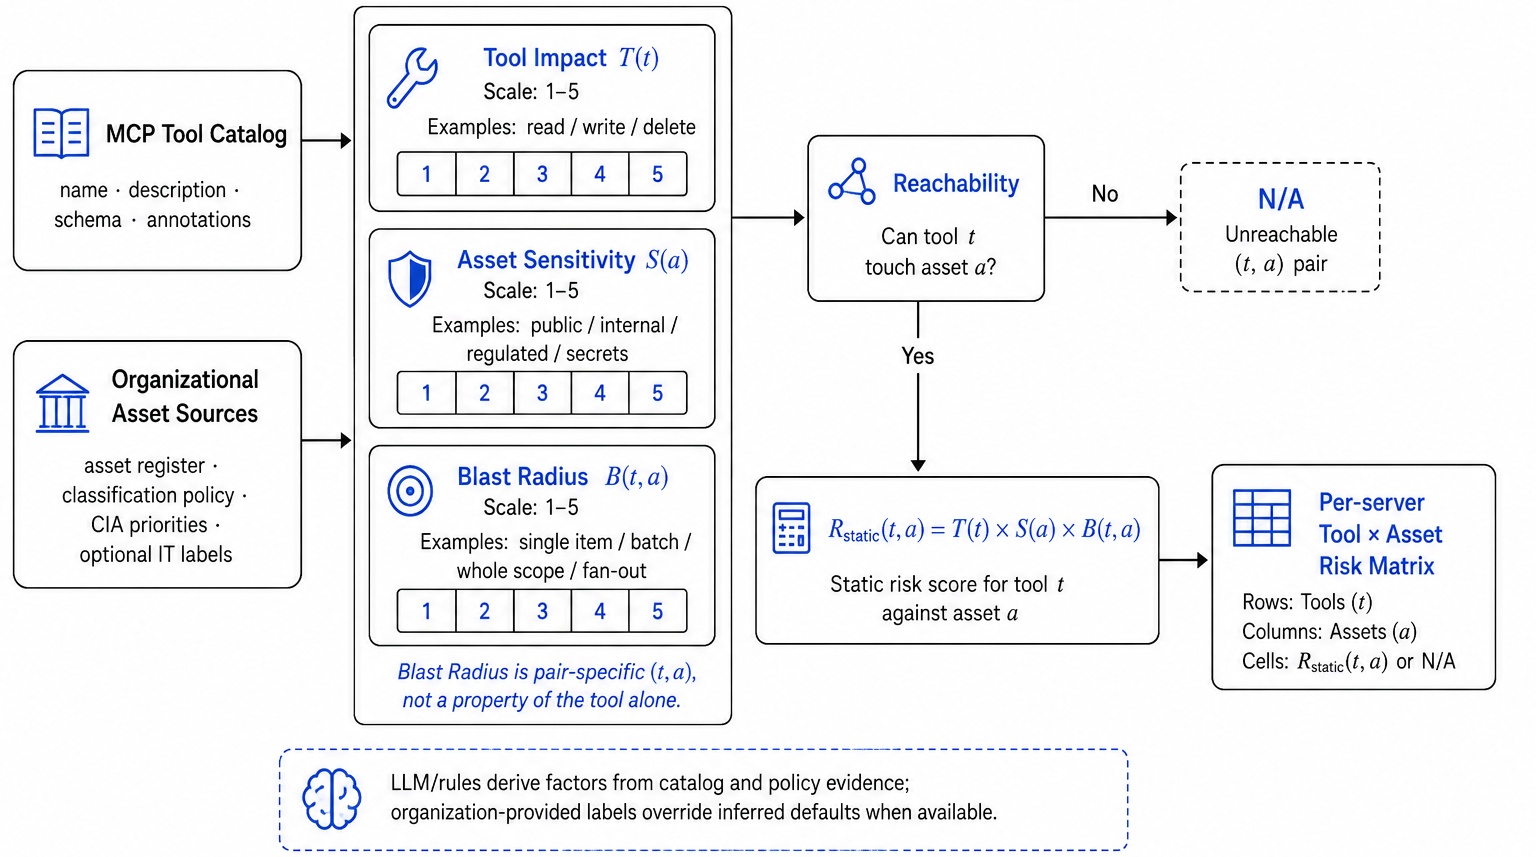
\includegraphics[width=\columnwidth]
    {figures/mcp_static_scanner_architecture_updated.png}
    \caption{Static Scanner. MCP tool information and organizational asset
    information are used to estimate tool impact, asset sensitivity,
    blast radius, and reachability. The output is a per-server
    tool--asset risk matrix.}
    \label{fig:static-scanner}
\end{figure}


% ---------------------------------------------------------------------------
\subsection{Static Layer}
\label{sec:impl-static}

The Static Scanner takes the captured catalog for a server together with the
organization's asset register and classification policy, and produces the
matrix $\mathbf{R}_{\mathrm{static}}$.

\textbf{Reachability.} The register states which tools may address which
assets, and schema constraints narrow that further. Pairs left unreachable are
emitted as \emph{N/A} and never scored, which is what produces the large
non-applicable fraction reported in Section~\ref{sec:results}.

\textbf{Tool impact $T(t)$.} Impact is resolved by a deterministic operation
ladder first, with a semantic classifier used only where the ladder abstains.
The ladder applies a strict evidence precedence. MCP tool annotations are
consulted first, but only as far as the specification licenses them: the
destructive and idempotent hints are meaningful only when the read-only hint is
false, and all of them are hints supplied by a possibly untrusted server. An
annotation may therefore \emph{bound} a tier --- a declared read-only tool
cannot exceed content access --- but no annotation on its own promotes a tool
to the top tier. Within that bound, verb evidence in the tool's name and
description decides, and a tool spanning several tiers takes the highest one it
reaches. Parameters describe but do not decide: a raw-query parameter, an
outbound-send parameter, or an unconstrained path is recorded as a capability
flag only, because what a parameter \emph{could} carry is a design-time
possibility while what a given call \emph{does} carry is a runtime fact
belonging to the dynamic layer. Every classification returns the evidence that
produced it, and the scorer that decided each tool is recorded, which is what
allows the deterministic and semantic shares to be reported separately.

\textbf{Asset sensitivity $S(a)$.} The policy states adverse impact per class
and carries no numbers, so the organization is never asked to supply a
per-asset risk score.

\textbf{Blast radius $B(t,a)$ and banding.} The score is the product of the
three factors, and the reporting bands of Section~\ref{sec:risk-output} are a
deterministic function of the primitives --- no second model call assigns a
band.

An earlier version of the pipeline ran an additional reviewer stage in which an
independent model re-derived each primitive and could override the first. We
removed it from the scan path: measured against the deterministic assignment it
altered roughly 46\% of bands, inflated the Critical band severalfold, and made
matrices irreproducible across runs. Its useful contribution was made permanent
instead of per-run, by folding its band-level corrections into the deterministic
banding rules and its skepticism into the primitive prompts. The reviewer is
retained for evaluation only, to measure how often an independent model agrees
with the scanner, and is never invoked during a scan.


% ---------------------------------------------------------------------------
\subsection{Dynamic Risk Adaptation}
\label{sec:dynamic}

The static score captures the potential consequence of a capability, but two
invocations of the same tool on the same asset need not present the same
runtime situation. Concrete arguments, requested scope, timing, and previous
behavior of the caller provide additional evidence about the current
invocation.

For each incoming invocation, the Dynamic Scanner first resolves the target
asset and requested scope, and retrieves the corresponding
$R_{\mathrm{static}}(t,r)$.

The Dynamic Scanner maintains a behavioral state based on previously completed
invocations. This state includes expected tools, parameter distributions,
invocation frequency and recency, and sequences of tool use.

The Dynamic Scanner then evaluates request-time evidence using three factors:

\textbf{Baseline Deviation ($D$).}
This factor captures how much the current invocation differs from previously
observed behavior, such as changes in tool use, parameter values, frequency,
or invocation sequence.

\textbf{Access Anomaly ($A$).}
This factor captures how unusual the requested access is for the target
asset, including unusual targets or requested scope.

\textbf{Novelty and Exposure ($N$).}
This factor captures how new or rarely observed the current combination of
tool, asset, and parameters is.

Each factor ranges approximately from $1$ to $2$, where values near $1$
represent familiar behavior and larger values represent stronger evidence of
unusual or new behavior. We combine these factors into the bounded runtime multiplier:
\begin{equation}
L(c)=D(c)\,A(c)\,N(c),
\label{eq:runtime-factor}
\end{equation}
so that $L(c)$ ranges approximately from $1$ to $8$.

The final assessment is

\begin{equation}
R_{\mathrm{dynamic}}(c)
=
R_{\mathrm{static}}(t,r)\,L(c).
\label{eq:dynamic-risk}
\end{equation}

This formulation assigns different responsibilities to the two layers.
$R_{\mathrm{static}}$ represents the potential consequence of the capability,
whereas $L(c)$ represents evidence specific to its current use. Because the
runtime factors are bounded below by $1$, familiar behavior does not reduce
the static risk, while unusual or new behavior can increase the assessment.

The dynamic state evolves as invocations are observed. Information from
completed invocations, such as outcomes, errors, latency, sequences, and
timestamps, is added to the runtime history. Recurring behavior can become
established over time, while changes in scope, frequency, target, parameters,
or invocation sequence can raise the assessment again.

\begin{figure}[t]
    \centering
    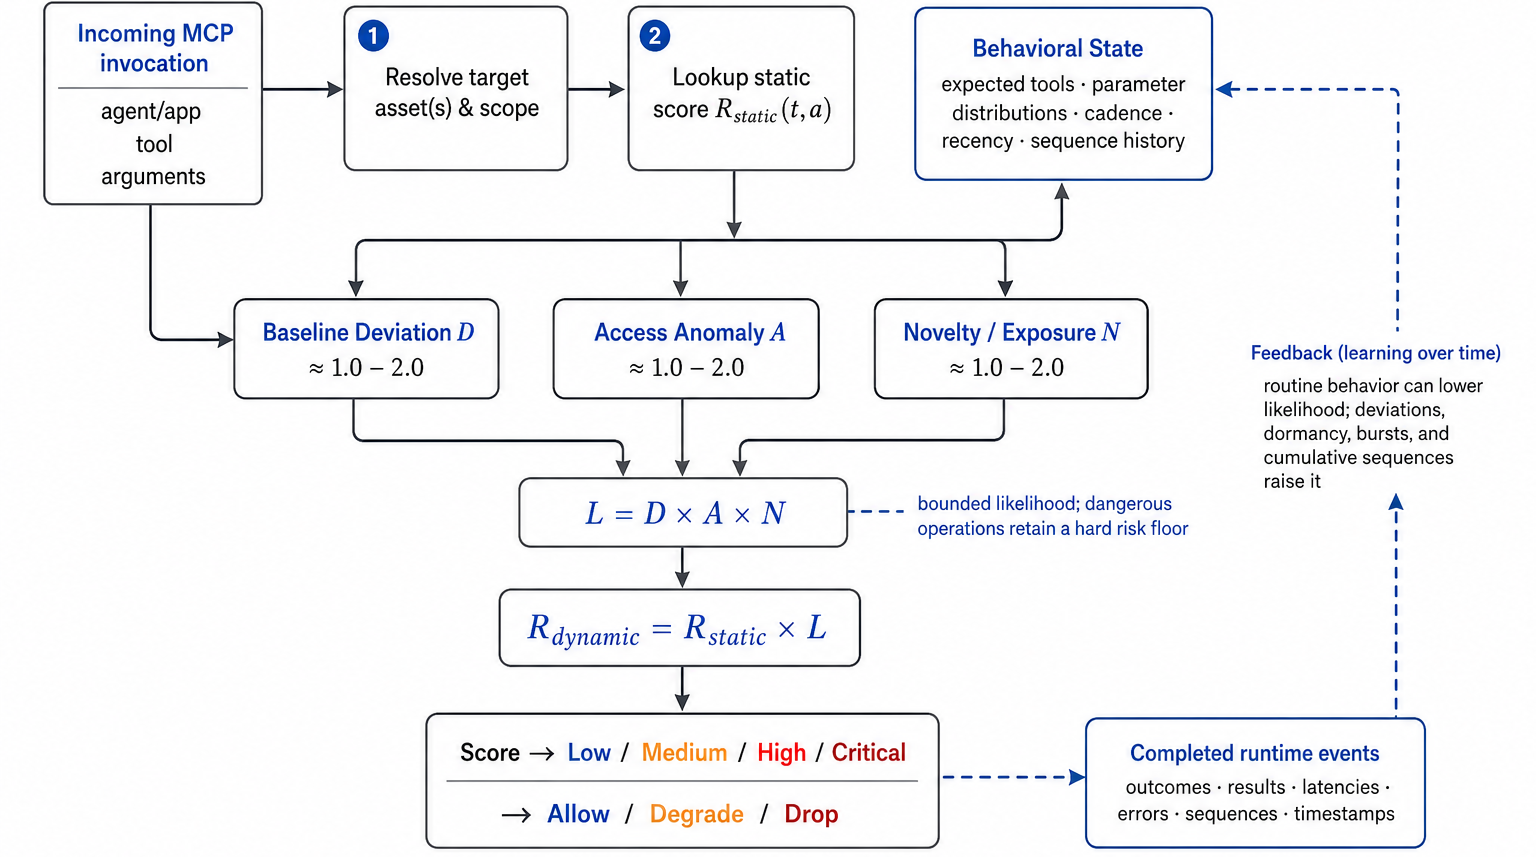
\includegraphics[width=\columnwidth]
    {figures/mcp_dynamic_scanner_architecture_updated.png}
    \caption{Dynamic Scanner. A concrete invocation is matched with its
    static tool--asset score and adapted using baseline deviation,
    access anomaly, novelty/exposure, and previously observed behavior.}
    \label{fig:dynamic-scanner}
\end{figure}


% ---------------------------------------------------------------------------
\subsection{Dynamic Layer}
\label{sec:impl-dynamic}

The Dynamic Scanner runs in front of the server and must return a verdict
before the invocation proceeds. This imposes a hard constraint that shapes the
whole implementation: \emph{no model runs on the invocation path}. Every
mechanism below is deterministic Python --- table lookup, pattern matching, and
weighted token overlap --- and the design-time output of
Section~\ref{sec:impl-static} reaches it only as artifacts already on disk. A
verdict therefore costs no inference, reproduces exactly, and cannot be steered
by text an attacker writes into an argument.

\textbf{Resolving the target asset.} A tool is not one action; it is one action
per container it can address, and the argument chooses. The resolver turns
$(t, \text{arguments})$ into the set of register assets the call reaches, and
does so without any per-server configuration. Which argument names a container
is discovered from observed traffic by successive elimination: the argument
must take values from a bounded set, must be reused across calls rather than
minted anew each time, must carry handles rather than natural-language phrases,
must be accepted by more than one tool, and its values must map close to
one-to-one onto register rows. The verb that enumerates those containers is
whichever tool's output contains their identifiers, with the human-readable name
read from the text nearest the identifier and a binding accepted only when most
occurrences agree. Where nothing enumerates, the resolver falls back to
classifying what calls against an identifier returned, counting only tokens that
distinguish one container from its siblings.

The resolver is deliberately conservative. An identifier that nothing binds
returns the closure over every container the tool can reach, explicitly flagged
as unresolved, rather than a low-risk guess --- guessing low is how a gate is
walked past. It also returns a set rather than a single asset, because an
operation such as updating a calendar event genuinely touches the calendar, the
event record, and the attendee list at once.

\textbf{Baseline deviation ($D$).} The behavioral state is a profile per
(persona, server) pair built only from that persona's own observed calls: the
set of tools it has used, the highest asset sensitivity it has reached, and the
mean and standard deviation of its session sizes. There is no labeled training
data and no external benchmark. A call deviates when it uses a tool this persona
has never used, when it touches an asset more sensitive than any it has touched
before --- escalating with the size of the gap --- or when its session is
statistically larger than this persona's own norm. Where no history exists, the
implementation reports no signal rather than fabricating one.

\textbf{Access anomaly ($A$).} This factor asks about the objective rather than
about the agent: does the call attack the confidentiality, integrity, or
availability objective that the organization named as this asset's primary
loss? Both inputs are lookups --- the objective a given operation violates comes
from the operation classification computed at design time, and the objective an
asset protects is the leading axis of its register entry, parsed once per
server. We found that treating this as an independent escalator fired on
between half and two-thirds of all cells and swamped the bands, so it is
applied instead as a
\emph{qualifier}: it can withhold an escalation the behavioral signals would
otherwise apply, but can never introduce one. A call that is off-axis is left
exactly where the static scan placed it.

\textbf{Novelty and exposure ($N$).} Novelty is carried by the unseen-tool and
above-prior-maximum conditions of the persona profile, together with the one
signal that inspects call \emph{order}: a read of a highly sensitive asset
followed within a short window by an outbound-capable call. Neither call need be
individually alarming; the sequence is the evidence, and no per-call or
per-cell view can see it.

\textbf{Composition.} The runtime factors of Equation~\ref{eq:runtime-factor}
are realized over the discrete reporting bands rather than as continuous
multipliers: each signal proposes a band and the final verdict is the most
severe proposal, qualified as described above. This keeps the bounded-below
property of Equation~\ref{eq:dynamic-risk} noted above intact. An optional
model-based reviewer that inspects concrete arguments can be enabled for
offline analysis; when it is not run this is recorded explicitly rather than
being treated as a clean verdict, and it is disabled by default so that the
invocation path stays model-free.

Every verdict retains each contributing signal separately alongside the final
band --- the static floor, the deviation, the sequence, the objective
qualification --- so that an assessment can be explained in terms of the
evidence that produced it rather than presented as a single opaque number. The
per-stage timings recorded by both layers provide the measurement points for
the operational properties evaluated in Section~\ref{sec:operational-eval}.


% ---------------------------------------------------------------------------
\subsection{Risk Output}
\label{sec:risk-output}

The output of the framework is the graded dynamic assessment
$R_{\mathrm{dynamic}}(c)$ together with the factors that contributed to it.
An organization may map this value to its own risk bands or use it as input
to logging, review, or access-control mechanisms.

For the static characterization reported in
Section~\ref{sec:results}, we use four reporting bands on the $1$--$125$
static scale: \emph{Low} for scores below 17, \emph{Medium} for scores from
17 to 49, \emph{High} for scores from 50 to 99, and \emph{Critical} for
scores of 100 or greater. These bands are used to summarize the experimental
risk surface and do not prescribe an enforcement policy.

We deliberately separate assessment from enforcement. The framework estimates
the risk associated with executing an invocation; the organization determines
what action, if any, should follow according to its own risk tolerance.


\section{Evaluation}
\label{sec:evaluation}

Our evaluation studies whether the proposed method produces different and
explainable risk scores across MCP environments, and whether the dynamic layer
can be used on real invocation traces.

No existing benchmark evaluates MCP risk at the granularity considered in this work. Prior MCP and agent-security approaches assess different objects, including server-level risk, tool-level risk, and request-level safety~\cite{kumar2026mcpinsos,betser2026agentrim,zhang2026stars}, and therefore do not provide a comparable reference for tool--asset or invocation-level risk estimation. 

More fundamentally, there is no established ground-truth risk score for an authorized MCP invocation against which such estimates can be calibrated. Consequently, our evaluation does not treat risk estimation as a regression problem against a predefined "correct" score. Instead, we evaluate whether the proposed methodology produces consistent risk ordering, responds systematically to changes in individual risk factors, and adapts appropriately to runtime behavioral context.

% The preliminary results in
% Section~\ref{sec:results} focus on the static risk scores and on whether the
% runtime layer can be used efficiently during tool invocation. 


% A direct
% numerical comparison with previous approaches is difficult. Existing MCP and
% agent-security methods measure different types of risk, such as server-level
% risk, tool-level risk, or request-level safety
% ~\cite{kumar2026mcpinsos,betser2026agentrim,zhang2026stars}. Their scores
% therefore cannot be used as a direct reference for our tool--asset and
% invocation-level risk scores. There is also no single known numerical ground
% truth for the risk of an authorized MCP invocation. We therefore do not
% evaluate the framework by checking whether it predicts one ``correct'' score.
% Instead, we study the risk scores produced by the framework, how the different
% risk factors affect these scores, and properties that can be measured without a
% reference risk score.

\subsection{Evaluation Settings}
\label{sec:evaluation-setting}


We evaluate the framework on MCP server deployments from several application
domains. For each deployment, we obtain the tool catalog exposed through the
MCP interface and use the organization's data-classification policy to
determine the sensitivity of the assets that the server can access. Some
deployments use the same MCP tool catalog under different organizational
settings, allowing us to examine how organizational context affects the
resulting risk assessment.

For the static evaluation, the framework builds a tool--asset matrix for
each deployment and assigns a risk score to each reachable pair.

For the dynamic evaluation, we use invocation logs collected from the
deployments. These logs contain time-ordered MCP calls, including their
concrete arguments, targets, operation sequences, and previous invocation
history. They provide the runtime information used by the dynamic layer.





\subsection{Static Assessment}
\label{sec:static-eval}

The static evaluation studies the risk surface produced before runtime
behavior is observed. We examine the distribution of reachable and
non-applicable tool--asset pairs, the resulting risk bands, and
representative high-risk combinations across different MCP domains.

The three-factor decomposition further permits component-level inspection. In particular, we examine how tool impact, asset sensitivity, and blast radius combine across different MCP environments, and whether high-risk assessments can be traced to the evidence underlying these factors.

We evaluated 16 server deployments drawn from 9 distinct MCP tool catalogs.
Each catalog was captured from a running server through the protocol's
tool-listing interface~\cite{mcp2026spec} and used as exposed by the server.
GitHub, Slack, and calendar catalogs were each instantiated under two
organizations, while the filesystem catalog was instantiated under five
organizations with different asset registers.

In total, the scan covers 262 tools, 221 registered assets, and
3,615 candidate tool--asset cells. Asset sensitivity was derived from
the organizational classification policy (synthesized using NIST format ~\cite{nist2008sp80060}).


\subsection{Establishing an External Human Baseline}
\label{sec:human-annotation}

The static scoring layer evaluated above is graded, throughout this section, against benchmarks that are themselves derived from the project's own documentation: tool registries, asset registers, and organizational policy text that the scanner itself consumes. This is a real limitation. For none of the deployments we scan does a held-out, externally sourced numeric ground truth exist for tool impact, asset sensitivity, or blast radius; when we vary only the policy framework under which the same deployment's sensitivity register is described -- ISO, NIST, or CIS wording for an otherwise identical asset -- scores for that asset can shift by as much as three tiers (e.g.\ a rating of $5$ under an ISO-styled policy against $2$ under a NIST-styled one and $5$ again under CIS). Such a shift is consistent with two very different explanations: either the source documents genuinely license different sensitivity judgments, in which case there is no single correct label to grade against, or the scanner is misreading policy language it should treat as equivalent. Nothing internal to the pipeline -- including an LLM judge re-reading text produced by an LLM-oriented policy generator -- can adjudicate between these two possibilities. Doing so requires a rater outside the system entirely, which motivates the human-annotation study we describe below.

Because no external ground truth for these dimensions has previously been collected, the study we designed targets \emph{reliability} rather than \emph{validity}: it asks whether independent expert raters can agree with one another at all, not whether any particular number is the objectively correct one. This ordering is deliberate. A scanner that matches human raters only as often as human raters match each other is operating at the human ceiling, not failing; conversely, a claim of the form ``the scanner is accurate'' is not well-posed until we know how much inter-rater disagreement exists even before the scanner enters the picture. Reliability is therefore treated as a precondition for, rather than a substitute for, any validity claim about the scanner.

We designed and built a self-contained rating instrument, the \emph{MCP Risk Docket}, distributed to each rater as a single link requiring no account or local setup. The instrument covers three rated dimensions, and each rater is assigned exactly one of the three so that no individual's judgments are shared across dimensions. The Tool Impact task shows a rater only a tool's raw JSON definition and asks them to judge its impact; because this requires no specialized security background, any working developer is eligible, and the task takes roughly eight minutes. The Asset Sensitivity task shows a rater one asset-register row together with its associated policy paragraph and is restricted to raters with a security, compliance, or data-governance background, taking roughly ten minutes. The Blast Radius task presents a rater with a single tool--asset pair in the context of the tool, the asset, and the surrounding peer-server environment, includes an explicit not-applicable option, is restricted to security engineers, and takes roughly eight minutes. Within each task, a rater sees eight real, scored items interleaved with three blinded attention-check items -- eleven items in total, presented in an order shuffled independently per rater -- so that low-quality responses can be identified and excluded without the rater knowing which items are checks.

The rated items are drawn from five real MCP server deployments already used elsewhere in this work: \texttt{github\_helios} (26 tools), \texttt{slack\_vireo} (16 tools), \texttt{calendar\_aurora} (13 tools), \texttt{fs\_corp\_filesystem} (14 tools), and \texttt{finance\_tools} (17 tools, notable among the five for its own fail-open, public-data-oriented sensitivity policy). Drawing items from this fixed, already-scanned set of deployments lets the study probe agreement across a range of domains and policy postures without introducing any material the static scanner has not also been evaluated against.

The primary statistic is Krippendorff's alpha computed with an ordinal difference function and pooled within each dimension, with confidence intervals obtained by non-parametric bootstrap (bias-corrected and accelerated, $B=10{,}000$). We pre-registered decision thresholds for interpreting alpha ahead of data collection: $\alpha \geq 0.800$ is treated as reliable, $0.667 \leq \alpha < 0.800$ as tentative, and $\alpha < 0.667$ as unreliable. Falling in the unreliable band does not by itself indicate anything about the scanner; it is a signal to revise the rubric or the item bank for that dimension, and such a dimension would not be used as a confirmatory benchmark until reliability is re-established. The pilot recruits three raters for Tool Impact, five for Asset Sensitivity, and three for Blast Radius, with a confirmatory scale target of 72--120 rated items per dimension. To keep the study honest, we committed a full pre-registration -- frozen rubric text, a frozen item bank, fixed per-rater shuffle seeds, a fixed exclusion rule, and the exact alpha variant, not-applicable convention, and bootstrap procedure -- before recruiting a single real rater, and deposited it on a public registry. Recruitment draws on a security-professional network rather than general crowdworkers, with a planned honorarium of \$25--40 per completed task where budget allows. A rater who fails two or more of the three attention checks in their task has their entire response set excluded from the primary analysis, though they are still compensated in full.

Once responses exist, the scanner will be graded by treating it as an $(n{+}1)$-th rater added to the same pool. The primary, pre-registered test for doing so is a permutation test: we compare the change in pooled alpha produced by swapping the scanner in for one human rater against the empirical distribution of the same statistic produced by swapping one human rater for another. A simpler check -- whether the scanner's score for an item merely falls within the observed range of human scores for that item -- is retained only as an illustrative secondary statistic, since with as few as three to five raters per dimension such a range check is high-variance and can look misleadingly good or bad independent of whether the scanner is actually tracking human judgment.

This design yields an honest range of possible outcomes rather than a single expected result. If human raters agree with each other reliably and the scanner's swap-in effect on alpha falls within the empirical spread of human-to-human swap effects, the scanner's disagreement with experts is statistically indistinguishable from ordinary inter-rater disagreement, and a first accuracy-style claim becomes supportable. If human agreement is reliable but the scanner's swap-in effect falls outside that spread, the scanner diverges from expert judgment by more than experts diverge from each other -- a genuine validity gap rather than an artifact of task difficulty. And if human-to-human agreement itself falls below the pre-registered reliability threshold, neither of the above conclusions can be drawn, because there is no sufficiently reliable target left to grade the scanner against; in that case the informative outcome is that the rubric or item bank for that dimension needs revision before any scanner accuracy claim can be entertained. We treat this last outcome as a legitimate and reportable finding in its own right, not as a failed experiment.

As an optional extension, and not required to support the primary reliability claim, the same instrument could be used to ask whether the choice of policy framework moves a human rater the way it moves the scanner: raters would see the identical asset described under ISO-, NIST-, and CIS-styled policy text and we would test whether their sensitivity judgments shift across frameworks by an amount comparable to the up-to-three-tier shifts observed for the scanner. This second arm is planned but not yet scheduled.

As of this writing, the protocol and the live pilot instrument are complete and pre-registration-ready, and a recruitment and compensation plan is in place, but no rater has yet completed the study. No agreement statistics, alpha values, or accuracy figures for this experiment exist yet; we report the design here as planned methodology whose results will be reported once data collection concludes.


\subsection{Dynamic Assessment}
\label{sec:dynamic-eval}

The runtime evaluation studies the feasibility of applying the dynamic layer
to real MCP invocation traces. We exercise concrete deployments with
time-ordered calls and record the information required by
$f_{\mathrm{dyn}}$, including arguments, targets, call frequency, and
invocation history.

The preliminary evaluation focuses on whether the runtime evidence can be
collected and scored efficiently on the invocation path. A full assessment
against independently annotated misuse traces is left for subsequent
evaluation.


\subsection{Additional Properties}
\label{sec:operational-eval}

We additionally evaluate operational properties that do not require a reference risk score.

\textbf{Computational Cost.}
Because the Static Scanner uses LLM-based analysis to derive the static risk factors, we measure the total computational cost required to analyze a given MCP server and construct its tool--asset risk matrix.

\textbf{Runtime Latency.}
For the Dynamic Scanner, we measure the per-invocation latency introduced by risk computation, i.e., the time required to compute the dynamic risk score for an incoming MCP request before execution.

% \textbf{Coverage.}
% We measure the portion of the tool--asset space for which the framework can
% establish reachability and produce a risk assessment.

% \textbf{Traceability.}
% We examine whether each assessment can be decomposed into the tool-impact, asset-sensitivity, and blast-radius evidence that produced it.

% \textbf{Automation.}
% We measure how frequently deterministic analysis is sufficient and how often
% semantic inference is required.

% \textbf{Overhead.}
% We measure the computational cost of constructing the static risk surface and
% the latency introduced by runtime scoring.

% Together, these measurements characterize the behavior and operational
% properties of the proposed assessment without assuming an unavailable
% universal MCP risk score.



% ===========================================================================
% 6. Preliminary Results
% ===========================================================================

\section{Preliminary Results}
\label{sec:results}

Currently, we report only the results of the Static Scanner. This section presents the static risk surface produced by our framework from real MCP tool catalogs.

\subsection{Static Assessment Results}

\begin{table*}[t]
\centering
\caption{Static scan by deployment. \emph{Cells} denotes the Cartesian
tool--asset space; \emph{Scored} is the subset judged reachable.}
\label{tab:corpus}
\scriptsize
\resizebox{\textwidth}{!}{
\begin{tabular}{llrrrrrrrrr}
\toprule
&&&&&&&\multicolumn{4}{c}{Scored cells by band}\\
\cmidrule(lr){8-11}
Kind & Deployment & Tools & Assets & Cells & Scored & N/A &
Low & Med. & High & Crit.\\
\midrule
Filesystem & \texttt{fs\_fintech\_fs}
& 14 & 18 & 252 & 103 & 149 & 39 & 36 & 24 & 4\\
Filesystem & \texttt{fs\_medical\_clinic\_fs}
& 14 & 16 & 224 & 86 & 138 & 27 & 37 & 22 & 0\\
Filesystem & \texttt{fs\_corp\_filesystem}
& 14 & 16 & 224 & 87 & 137 & 36 & 26 & 21 & 4\\
Filesystem & \texttt{fs\_law\_firm\_fs}
& 14 & 15 & 210 & 89 & 121 & 33 & 43 & 13 & 0\\
Filesystem & \texttt{fs\_media\_studio\_fs}
& 14 & 16 & 224 & 111 & 113 & 63 & 36 & 12 & 0\\
\midrule
Github & \texttt{github\_real}
& 26 & 20 & 520 & 139 & 381 & 39 & 48 & 52 & 0\\
Github & \texttt{github\_helios}
& 26 & 19 & 494 & 126 & 368 & 29 & 46 & 47 & 4\\
Chat & \texttt{slack\_real}
& 16 & 20 & 320 & 101 & 219 & 37 & 48 & 6 & 10\\
Chat & \texttt{slack\_vireo}
& 16 & 15 & 240 & 62 & 178 & 18 & 38 & 5 & 1\\
Calendar & \texttt{calendar\_real}
& 13 & 16 & 208 & 68 & 140 & 22 & 27 & 14 & 5\\
Calendar & \texttt{calendar\_aurora}
& 13 & 17 & 221 & 71 & 150 & 14 & 33 & 18 & 6\\
SQL & \texttt{sqlite\_cbg\_sqlite}
& 5 & 11 & 55 & 37 & 18 & 13 & 13 & 7 & 4\\
\midrule
Finance & \texttt{finance\_tools}
& 17 & 6 & 102 & 27 & 75 & 18 & 9 & 0 & 0\\
Finance & \texttt{openbb}
& 30 & 5 & 150 & 36 & 114 & 23 & 12 & 1 & 0\\
Finance & \texttt{sec\_edgar}
& 21 & 6 & 126 & 27 & 99 & 24 & 3 & 0 & 0\\
Finance & \texttt{yahoo\_finance}
& 9 & 5 & 45 & 12 & 33 & 9 & 3 & 0 & 0\\
\midrule
\textbf{Total} & \textbf{16 deployments}
& \textbf{262} & \textbf{221} & \textbf{3,615}
& \textbf{1,182} & \textbf{2,433}
& \textbf{444} & \textbf{458} & \textbf{242} & \textbf{38}\\
\bottomrule
\end{tabular}}
\end{table*}

Table~\ref{tab:corpus} shows that 1,182 of the 3,615 candidate cells
(33\%) were scored, while 2,433 (67\%) were classified as not applicable.
Thus, the framework classifies the majority of the Cartesian tool--asset space as non-applicable, substantially reducing the set of tool--asset pairs for which a risk score is produced.

The proportion varies substantially by server structure. For example, the
five-tool SQL deployment leaves only 18 of 55 cells unreachable, whereas the
30-tool OpenBB deployment leaves 114 of 150 unreachable because many of its
tools expose narrow, specialized functionality.

Among the reachable cells, 444 are Low, 458 Medium, 242 High, and 38
Critical. High and Critical cells together account for approximately 24\% of
the scored surface and 7.7\% of the complete matrix.


Most tool-impact assignments are deterministic. Across the 151 distinct tools, the deterministic operation ladder assigned
impact to 127 tools (84\%), while semantic analysis was required for the
remaining 24. The split reflects differences in catalog vocabulary. Tools with
common operation semantics such as \texttt{get}, \texttt{search}, and
\texttt{list} are usually resolved directly, whereas domain-specific verbs
such as \texttt{fork}, \texttt{merge}, or \texttt{push} more often require
semantic interpretation.

This result is operationally useful because semantic inference is concentrated
on the ambiguous portion of the tool surface rather than being required for
every tool.


\subsubsection{Highest-Risk Combinations}

Table~\ref{tab:top} reports the highest-scoring tool--asset pair in each
deployment. The resulting combinations illustrate the interaction between the
three static factors: high scores arise when consequential operations,
sensitive organizational assets, and broad scope coincide.


\begin{table*}[t]
\centering
\caption{Highest-scoring tool--asset pair in each deployment.}
\label{tab:top}
\scriptsize
\resizebox{\textwidth}{!}{
\begin{tabular}{llcr}
\toprule
Deployment & Highest-scoring tool--asset pair &
$S\cdot B\cdot T$ & Score\\
\midrule
\texttt{fs\_fintech\_fs}
& \texttt{write\_file} $\times$ \texttt{card-vault}
& $5\cdot5\cdot4$ & 100\\
\texttt{fs\_corp\_filesystem}
& \texttt{write\_file} $\times$ \texttt{security-keys}
& $5\cdot5\cdot4$ & 100\\
\texttt{fs\_medical\_clinic\_fs}
& \texttt{write\_file} $\times$ \texttt{patient-charts}
& $5\cdot4\cdot4$ & 80\\
\texttt{fs\_law\_firm\_fs}
& \texttt{write\_file} $\times$ \texttt{matter-files}
& $5\cdot4\cdot4$ & 80\\
\texttt{fs\_media\_studio\_fs}
& \texttt{write\_file} $\times$ \texttt{unreleased-imagery}
& $4\cdot4\cdot4$ & 64\\
\texttt{github\_helios}
& \texttt{push\_files} $\times$ \texttt{helios-scada-gateway}
& $5\cdot5\cdot4$ & 100\\
\texttt{github\_real}
& \texttt{fork\_repository} $\times$ \texttt{infra-config}
& $4\cdot5\cdot4$ & 80\\
\texttt{slack\_real}
& \texttt{conversations\_leave} $\times$ \texttt{incident-response}
& $5\cdot5\cdot5$ & 125\\
\texttt{slack\_vireo}
& \texttt{usergroups\_users\_update} $\times$
  \texttt{usergroup-membership}
& $4\cdot5\cdot5$ & 100\\
\texttt{calendar\_real}
& \texttt{manage-accounts} $\times$ \texttt{connected-account-config}
& $5\cdot5\cdot5$ & 125\\
\texttt{calendar\_aurora}
& \texttt{delete-event} $\times$ \texttt{aurora-exec}
& $5\cdot5\cdot5$ & 125\\
\texttt{sqlite\_cbg\_sqlite}
& \texttt{write\_query} $\times$ \texttt{api\_keys}
& $5\cdot5\cdot5$ & 125\\
\texttt{finance\_tools}
& \texttt{calculate} $\times$ \texttt{expression-evaluator}
& $4\cdot3\cdot3$ & 36\\
\texttt{openbb}
& \texttt{install\_skill} $\times$ \texttt{server-capability-install}
& $4\cdot4\cdot4$ & 64\\
\texttt{sec\_edgar}
& \texttt{get\_recommended\_tools} $\times$ \texttt{concept-catalogs}
& $3\cdot3\cdot3$ & 27\\
\texttt{yahoo\_finance}
& \texttt{get\_historical\_stock\_prices} $\times$
  \texttt{research-query-pattern}
& $3\cdot3\cdot3$ & 27\\
\bottomrule
\end{tabular}}
\end{table*}


The organization-specific component is visible in the filesystem deployments:
the highest-scoring \texttt{write\_file} pair changes with the asset that
each organization's policy considers most consequential, including payment
data, security keys, patient information, legal matter files, and unreleased
media.

The public-data deployments provide the opposite case. The
\texttt{finance\_tools}, \texttt{sec\_edgar}, and
\texttt{yahoo\_finance} deployments produce no High or Critical cells across
their 273 candidate cells. This difference arises despite using the same
scoring methodology, illustrating the role of organizational asset context
rather than tool semantics alone.

The scan also grades every input parameter for how much stored data it alone
can reach, on a five-level scale, independently of whether the parameter
carries a numeric quantity: an identifier parameter has no magnitude, but it
still selects what is opened, so it still receives a grade. On the GitHub,
Slack, and Calendar catalogs used in the dynamic evaluation below, this
classification reached full coverage. All 303 parameters (130, 63, and 110,
respectively) were graded, with none left ungraded.








% ===========================================================================
% 7. Conclusion
% ===========================================================================

\section{Conclusion}
\label{sec:conclusion}

Authorization answers whether an MCP invocation is permitted; it does not
express how consequential that permitted invocation may be. We presented a
server-side framework for estimating this risk before execution.

The framework separates assessment into two layers. At design time, the Static
Scanner constructs a risk surface over reachable tool--asset pairs using
three interpretable factors: tool impact, organizational asset sensitivity,
and blast radius. Asset sensitivity is grounded in the organization's own
classification policy, following established security-categorization
principles~\cite{nist2004fips199,nist2008sp80060}. At runtime, the Dynamic
Scanner adapts the corresponding baseline using invocation-specific context
and previously observed behavior.

Our preliminary study covers 16 deployments of 9 real MCP tool catalogs,
comprising 262 tools, 221 organizational assets, and 3,615 candidate
tool--asset pairs. The framework identifies 67\% of this Cartesian space as
not applicable, while High and Critical pairs account for 7.7\% of the full
matrix. A deterministic operation ladder resolves 84\% of distinct tool-impact
assignments, limiting semantic inference to the ambiguous portion of the tool
surface. We additionally collected 3,000 live invocations across three
provisioned MCP deployments to exercise the runtime path.

A central property of the framework is that each assessment remains
decomposable. Rather than presenting an organization with only an opaque
number, the score can be traced to the operation, the organization's own
asset classification, the reachable scope, and the runtime evidence that
contributed to it.

The current results characterize the risk surface produced by the framework
rather than agreement with an independent universal notion of MCP risk.
Establishing agreement with organization-assigned severities and evaluating
the dynamic layer against independently annotated invocation traces are
therefore important directions for further evaluation.


\balance
\bibliographystyle{ACM-Reference-Format}
\bibliography{refs}

\end{document}
